\chapter{Úvod}
\section{Ozobot a jeho svět}
    Ozobot je komerčně dostupný, zhruba 2,5 na 2,5 centimetru velký robot, určený pro výuku základních principů programování. Robot se pohybuje díky dvěma malým elektromotorům, ovládajících každý jedno kolo robota. Elektromotory jsou řízeny deskou s~mikrokontrolérem, který kromě elektromotorů ovládá také LED diodu sloužící pro vizuální odezvu uživateli. Jediným interakčním prvkem je tlačítko na boku, sloužící k zapnutí a vypnutí robota.
    
    Ozobot je robot typu \uv{black line follower} - pokud Ozobot stojí na černé čáře o tloušťce minimálně 5 milimetrů, automaticky po ní pojede. K této funkci Ozobot využívá pět senzorů, které rozeznávají černou a bílou barvu. Pokud Ozobot nejede prostředním senzorem po černé čáře, ale po některém z bočních senzorů, Ozobot upraví svůj kurz tak, aby jel opět prostředním senzorem po čáře.
    
    Ozobot má navíc funkci patentovanou firmou Ozobot, která je klíčem k tomuto projektu - funkce Color Codes. Tato funkce umožňuje Ozobotu upravovat svoje chování, tedy jeho rychlost, směr jízdy, nastavení časovače a podmínek pro "výhru". Těsně před prostředním senzorem čáry je umístěn i se senzor barev citlivý především na rozlišení červené, zelené a modré. Pokud tedy Ozobot přejede přes kombinaci těchto tří barev v tří až čtyřčlenné sekvenci, robot upraví svoje chování podle dané sekvence (viz obr. \ref{fig:color-codes} Tabulka sekvencí).
    
    Firma Ozobot nabízí způsob použití těchto sekvencí dvěma způsoby - Barevnými fixy, nebo samolepkami, obojí je dostupné od řečené firmy k zakoupení.

\begin{figure}[h!]
          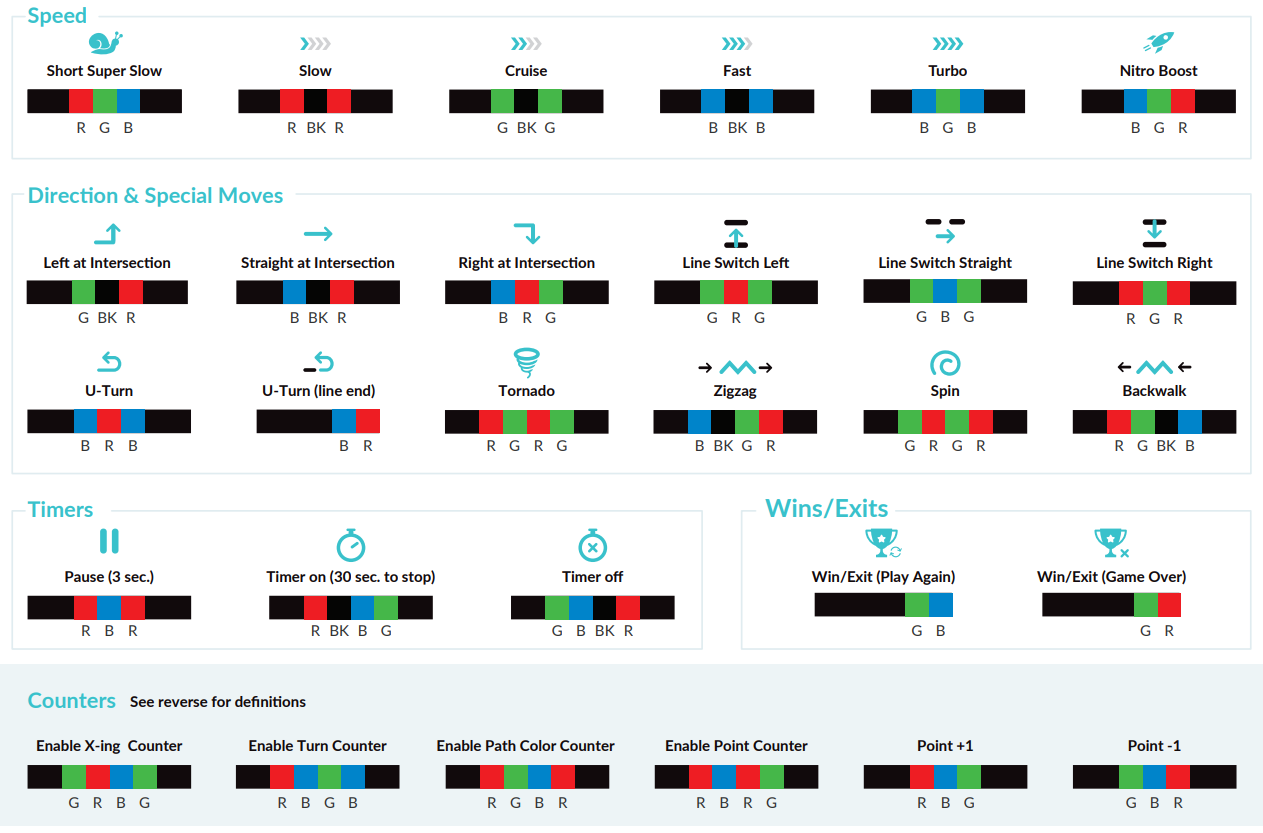
\includegraphics[width=\textwidth]{images/color_codes.png}
          \caption{Tabulka sekvencí.}
          \label{fig:color-codes}
        \end{figure}

\section{Existující řešení}
    Ozobot je uzpůsoben jízdě po papíru, a podle toho tudíž existují předem zmiňované způsoby aplikace barevných sekvencí, tedy barevnými fixy a samolepkami. Krom tohoto standardního způsobuje existuje alternativa, a to v podobě tabletu s nainstalovanou aplikací. Ta může být přímo určená pro platformu Ozobot, např. Ozogroove, stačí ovšem i obyčejná aplikace typu \uv{plátno}, např. Sketchbook, nebo Infinite Painter.
    